En el momento que sigue en la simulación, la porción de la energía cinética de la gráfica circular disminuye, entonces:

\begin{minipage}{0.3\textwidth}
    \begin{figure}[H]
        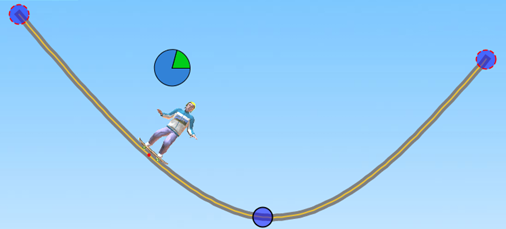
\includegraphics[width=\linewidth]{../images/q028c}
    \end{figure}
\end{minipage}\hfill
\begin{minipage}{0.6\textwidth}
    \begin{choices}
        \choice El patinador va mas rápido
        \choice El patinador va mas lento
        \choice No hay manera de saberlo
    \end{choices}
\end{minipage}
